\documentclass[10pt,a4paper]{article}
\usepackage[utf8]{inputenc}
\usepackage{amsmath}
\usepackage{amsfonts}
\usepackage{amssymb}
\usepackage{graphicx}
\usepackage{subfigure}
\usepackage{amsmath}
\usepackage{mathrsfs}
\DeclareRobustCommand{\orderof}{\ensuremath{\mathcal{O}}}
\bibliographystyle{prsty}
\usepackage[top=1in, bottom=1in, left=1in, right=1in]{geometry}

\begin{document}
\section{Introduction}
\textbf{scc} is the last part of the core level. It performs the self-consistent TB+U calculation and calculate the Fermi-level of the system. Even though you are not going to deal with a TB+U problem, it it still necessary to run this task because it still contains other necessary information to perform tasks in application level.

\section{Dictionary}

\subsection{Input}
\textit{\textbf{scc.HubU}} This parameter sets the Hubbard U of each state. To give U on a state, just input the state label and its Hubbard U, e.g [1,2;2,2] means state 1 and 2 both have Hubbard U=2. Here we only consider the direct Hubbard term which reads $H_{Hub}=Un_{i}n_{i}$ no matter what basis you are using. This is equivalent to consider the $F_{0}$ Slaster integral only in full Hubbard potetial calculation. You can leave this parameter empty if you are not going to perform TB+U calculation. \\ \\
\textit{\textbf{scc.Charge}} This parameter sets the initial charge distribution of the self-consistent iteration. Just input the average charge number of each state. If no TB+U calculation is performed, the distribution doesn't matter because system will get the correct distribution after one iteration. However, their sum, i.e. the total charge, has to be correct because it affects the position of Fermi level. If there are three states, then [0.6,0.4,1] means each their initial average charge is 0.6, 0.4 and 1 respectively. \\ \\
\textit{\textbf{scc.Mixing}} This parameter sets the mixing parameter of self-consistent iterations. The relation between the new and old density matrix is: $\rho_{new}=(1-\alpha)\rho_{in}+\alpha \rho_{out}$. scc.Mixing gives the value of $\alpha$.\\ \\
\textit{\textbf{scc.Iteration}} This parameter sets the maximal number of iterations. If self-consistency is not reached after the maximal loops, PiLab will stop. \\ \\
\textit{\textbf{scc.Converge}} This parameter sets the criterion of self-consistency. Once the absolute values of the difference between output and input density matrices are smaller than it, self-consistency is reached. \\ \\  
\textit{\textbf{scc.Mesh}} This parameter tells PiLab how to mesh the k-space. For example, [10,15,20] means to divide the reciprocal $b_{1}$, $b_{2}$ and $b_{3}$ into 10, 15 and 20 equal parts. The more dense of the grid, the more accurate Fermi level you will get. For insulator, you can use less dense grid. However, for metal, dense grid is needed. In most calculation, you might not care about the accuracy of Fermi level. If so, just input a very sparse grid, say [10,10,10].\\ \\
\textit{\textbf{scc.Temperature}} This parameter sets the temperature of the Fermi-Dirac distribution when calculating the Fermi-level. For insulator, it usually requires a larger value to get accurate result. This parameter doesn't mean an excitation calculation. It is just a parameter to estimate the Fermi-level. By default, PiLab sets it 100 which should be appropriate for most cases.\\ \\
\textit{\textbf{scc.Memory}} This parameter tells PiLab how to use the memory. If your scc.Mesh is very large, then the memory might not enough to store all calculation results. In this case, you will need to tune this parameter. By default, this parameter is set to 'normal'. If you find error message about memory, change it to 'max'. If it is still not working, set it to 'HDD'. HDD will use the hard disk to temporarily store calculated data which will lead the calculation very slow. Therefore, unless needed, it is strongly recommend to use a reasonable mesh, so that 'nomral' or 'max' are already enough.
  

\subsection{Output}
\textit{\textbf{scc.E\_Fermi}} This variable gives the Fermi level. For metal, this result is reliable only if scc.Mesh is dense enough. You can check its accuracy by observing the convergence of  the Fermi level when varying scc.Mesh. \\ \\
\textit{\textbf{scc.E\_gap}} This variable gives the band gap. Note that, even for metallic system, it may still gives a small gap due to enviably numerical error. The same, this result is reliable only if scc.Mesh is dense enough. \\ \\
\textit{\textbf{scc.DM\_out}} This variable outputs the self-consistent density matrix. Note that, \textbf{this variable will automatically be reloaded as the initial input density matrix every time scc is performed}. Therefore, if you keep it or manually change this variable, \textbf{scc} will ignore scc.Charge and use it as initial input automatically. \\ \\ 
\textit{\textbf{scc.U\_mat}} This variable gives the Hubbard potential. Since we only consider direct coulomb, this Hubbard potential matrix is always diagonal no matter in what basis as mentioned before.\\ \\ 
\textit{\textbf{scc.H\_onsite}} This variable gives the full onsite Hamiltonia. $H_{onsite}=hop.onsite\_E+hop.LS\_mat+scc.U\_mat$

\begin{figure}[tbp]
\centering
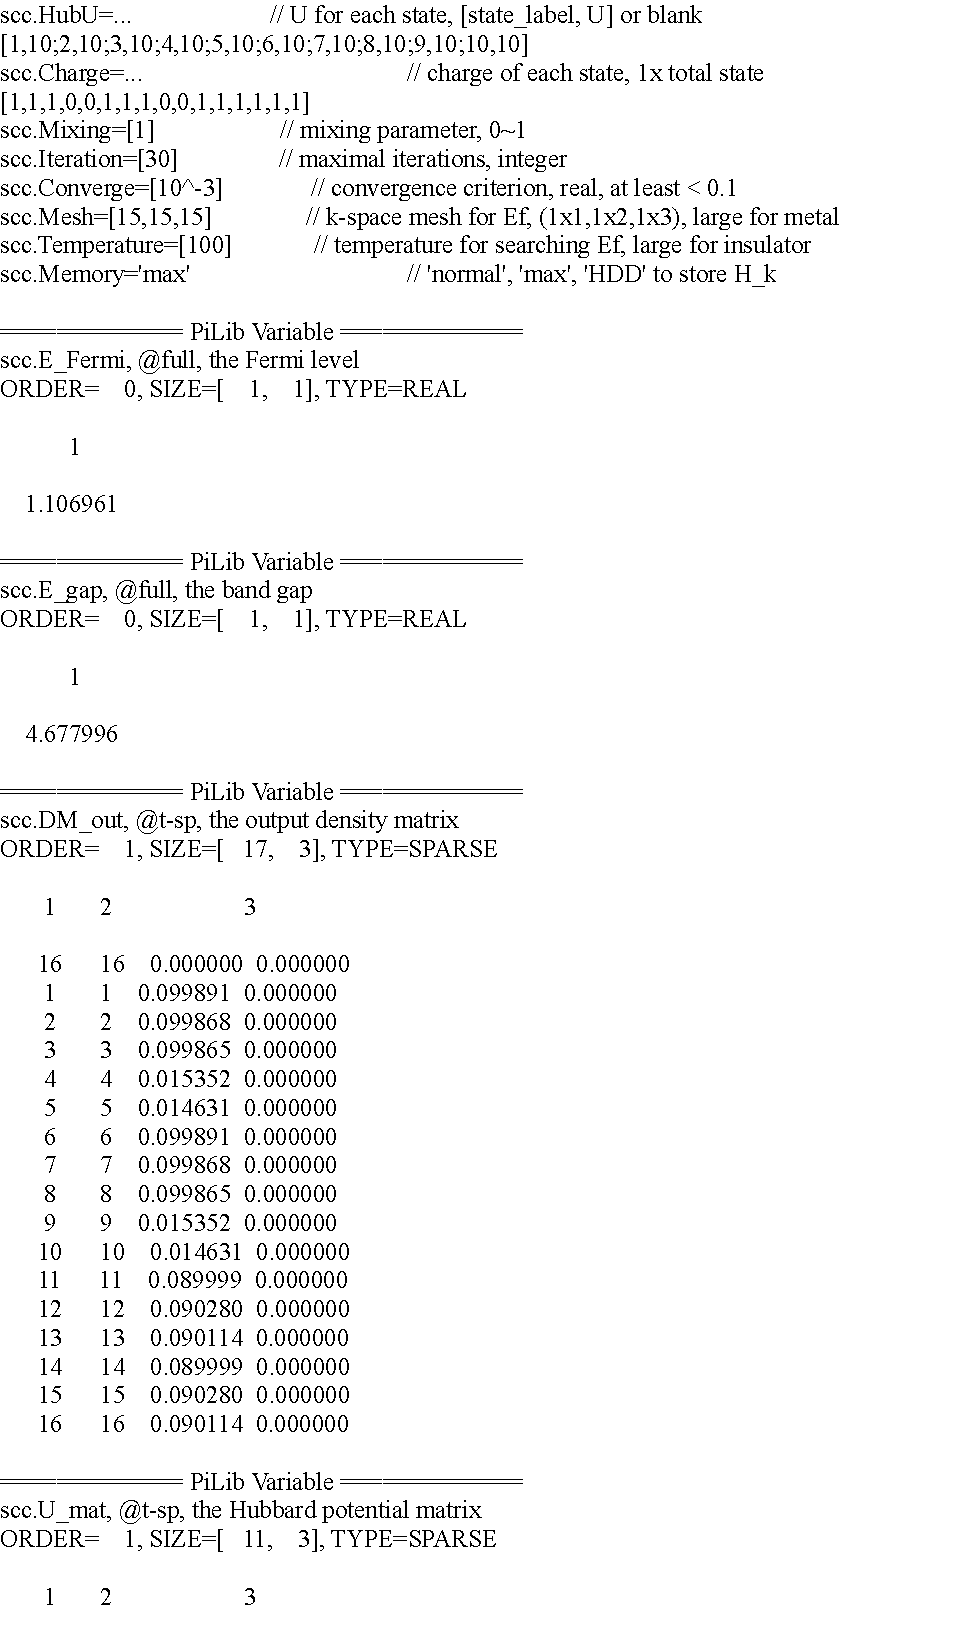
\includegraphics[width=0.9\columnwidth]{NiO_scc_p1.pdf}
\caption{page 1 of NiO\_scc.plb}
\end{figure}

\begin{figure}[tbp]
\centering
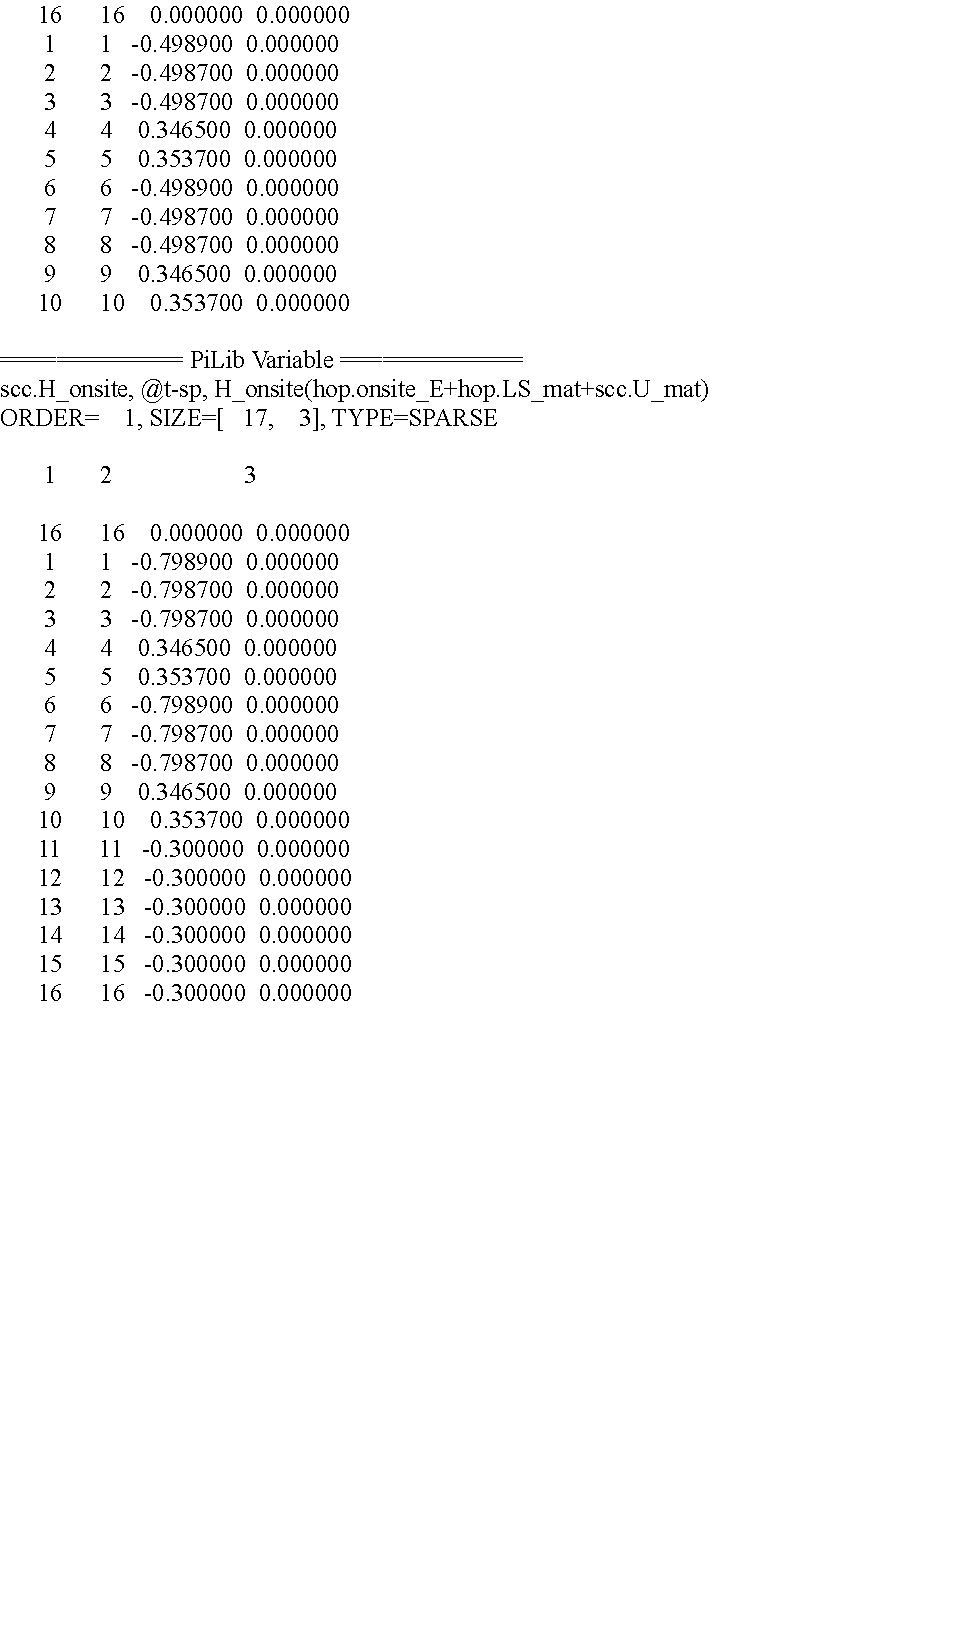
\includegraphics[width=0.9\columnwidth]{NiO_scc_p2.pdf}
\caption{page 2 of NiO\_scc.plb}
\end{figure}

\end{document}